\documentclass[10pt,a4paper,titlepage]{book}
\usepackage[latin1]{inputenc}
\usepackage{amsmath}
\usepackage{amsfonts}
\usepackage{amssymb}
\usepackage{makeidx}
\usepackage{multicol}
\usepackage{graphicx}
\author{Emin Topalovic}
\title{Interesting Algorithms}
\begin{document}
\maketitle
\pagenumbering{arabic}

\section{Algorithms and Geometry}
\subsection{Bresenham's Line Algorithm}
\subsubsection{Motivation}
Employing a graphics system of any sort requires the ability to work with basic shapes such as lines, triangles, and circles. We have formulas for graphic these on planes, and computers are good at computing, so we have the problem solved. Right? Well, one issue specific to computers is working with the constraint that our canvas is discretized. Since the computer screen works in pixels that are only ever in a binary state (on/off) we can't really draw point $(2.34, 5.6)$. After all, what would $.34$ of a pixel really mean? \\\\

This problem becomes more apparent when thinking about a specific application. For the purposes of this algorithm we will consider lines. Most of us know that one of the basic properties of a line is its $slope$ or rise-over-run. It would be very tempting to try and just use two points and their slopes and then to draw the pixels in a line based off of that. Let us, in fact, try to do just that. Say you have the point $(0,0)$ and point $(3,3)$. The slope here is $1$ so you draw the pixel at point $(0,0), (1,1), (2,2),$ and $(3,3)$. There, you have drawn the line and your method works, right? Well, think about this case. You have the point $(0,0)$ and $(3,2)$. The slope here is $\frac{2}{3}$ so you draw $(0,0), (1,\frac{2}{3}), (2, 1\frac{1}{3}),$ and $(3, 2)$. But wait, we already saw that $\frac{2}{3}$ of a pixel does not make sense, so we're stuck. How do we draw a line if we can't use real numbers? Like with most solutions in computer science, we find a way to solve our problem by finding the best approximation to the ideal solution. This is exactly what Bresenham's Line Algorithm does: it finds a way to draw a line in a $good$ $enough$ manner, or rather, in a manner whose faults are imperceptible to the user.       

\subsection{The Algorithm}
The main idea behind Bresenham's algorithm is that in trying to get from a point $(x_1, y_1)$ to a point $(x_2, y_2)$ we can choose to make steady progress along one axis while using this choice to determine whether or not we will progress in the other. More concretely, we can choose to always move from $x_1$ to $x_2$ in steps of $1$ pixel, and at each increment of $x$ decide whether or not to increment $y$. A run of the algorithm is reproduced below: \\\\
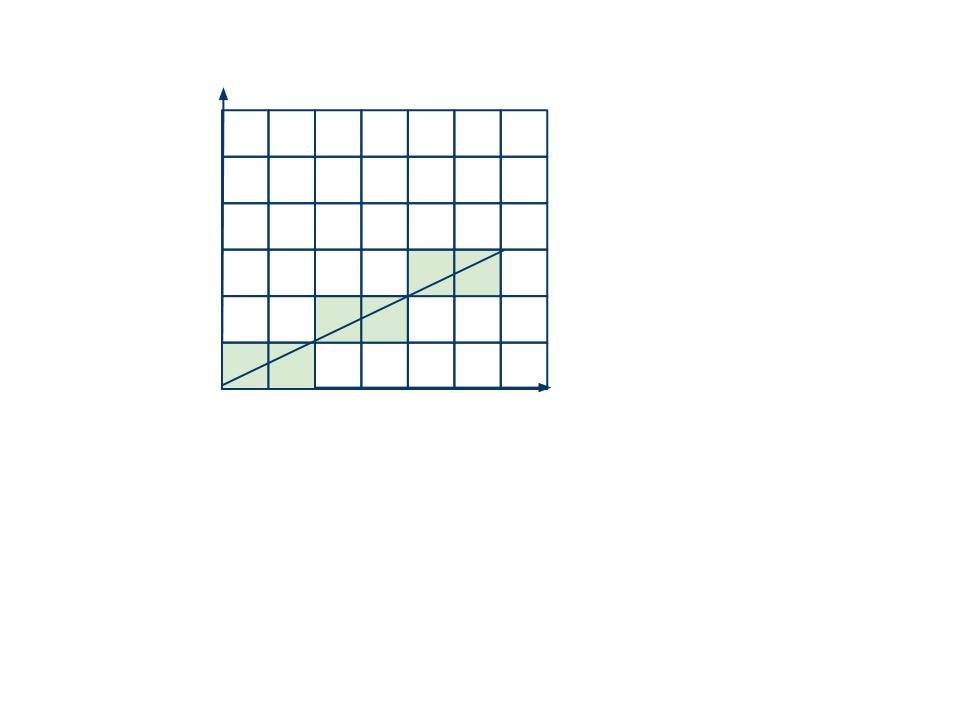
\includegraphics[bb=0 0 400 400,scale=.5]{imgs/BresenhamsLineAlgorithm.jpg}\\
The line clearly looks a little jagged, but we are leveraging the fact that the actual individual pixels are actually indistinguishable and therefore we do not notice the discontinuities.\\\\
The next natural question is how do we decide when to move up or down one pixel. For this we maintain a notion of an $error$ $term$ which expresses a relation of between our approximated location of the non-constant axis and where we would be were we using real numbers. For example, if the slope were $.5$ and we had just moved from $(0,0)$ to $(1,0)$ then we would have an error term of $.5$ since our location of $0$ is $.5$ away from where we would be on the line expressed over the real numbers. \\\\
Thus to pull the algorithm together we say that we will start the the $lower$ of the two points, increment one axis by $1$ keeping track of the y value produced as a result of the slope, and when our calculated slope exceeds the $error$ $term$ we increase by one in the other axis. A few details are clearly missing though. For instance, what do we mean by $lower$? This will actually be determined by how we choose our constant-increase axis. So, how should we do that? Well, we want to keep the slope of the line small, namely $<1$ so that every change of the slope does not trivially incur a change in the both axis (if it does you may run past your point!). If our slope is $>1$ we observer that we can make it $<1$ by reflecting the line along $y=x,$ or more concretely by making our y-axis the constant axis. Therefore which constant axis we use depends on the slope of the desired line. This, then lets us determine the $lower$ point by saying it is the point whose $x$ or $y$, depending on the constant axis, is the minimum between the two points.\\\\
This algorithm is fairly simple but powerful. It gets even more powerful when you realize that the whole thing can be done with integral numbers and without any multiplication or division. The specifics I will leave up to you, but I will present the insight here. One of the he points where you feel you might have to use division would be the slope of the proposed line; this, however, can be kept by considering each of the respective values composing the slope (rise and run) individually. You might also be tempted to think you need floating point to represent the error, but consider the following. We update our error as follows: \[\epsilon + \frac{dx}{dy} < \frac{1}{2} \] We can remove the right fraction by scaling by two: \[2\epsilon + 2 \frac{dx}{dy} < 1\] We can then remove the slope fraction by scaling by $dy$: \[\epsilon*dy + dx < dy\]
The multiplication we can remove by doing the times two multiplication using bitwise operations. We also notice that we don't have to explicitly do the $error$ $term$ multiplication and just view this as our error term scaled. 
\end{document}
